\documentclass[12pt]{article}
\usepackage[top = 2.5cm, bottom = 2.5cm, left = 2.5cm, right = 2.5cm]{geometry}
\usepackage{listings}
\usepackage{color} % red, green, blue, yellow, cyan, magenta, black, white
\usepackage{amsmath}
\usepackage{amssymb}
\usepackage{bm}
\usepackage{enumerate}
\usepackage{graphicx}
\usepackage{float}
\usepackage{booktabs}
\usepackage{makecell}
\usepackage[hidelinks]{hyperref}
\usepackage{multicol}
\usepackage{multirow}
\usepackage{cite}
\usepackage{bbding} % checkmarks
\usepackage{fancyhdr} % change the position of page number
\usepackage[flushleft]{threeparttable} % footnote in tables
\usepackage{lipsum}
\usepackage{caption}
\captionsetup{format = hang}
\usepackage{color, colortbl} % coloring rows or columns in tables
\definecolor{Gray}{gray}{.9} % coloring rows or columns in tables
\definecolor{darkgreen}{RGB}{0,100,0}
\definecolor{darkred}{RGB}{100,0,0}
\newcommand{\horrule}[1]{\rule{\linewidth}{#1}}
\fancyhf{} % clear all header and footers
\renewcommand{\headrulewidth}{0pt} % remove the header rule
\rfoot{\thepage} % puts the page number on the right side
\pagestyle{fancy}
\title{Spider plots}
\date{\today}
\author{Henrique Laureano\\
        \texttt{https://henriquelaureano.github.io/}}

\begin{document}

\maketitle
\thispagestyle{empty}

%\vfill
\noindent \horrule{.5pt} \vspace{-.95cm} \tableofcontents \noindent \horrule{.5pt}

\section*{Coefficients}
\addcontentsline{toc}{section}{Coefficients}

\begin{figure}[H]
 \centering
 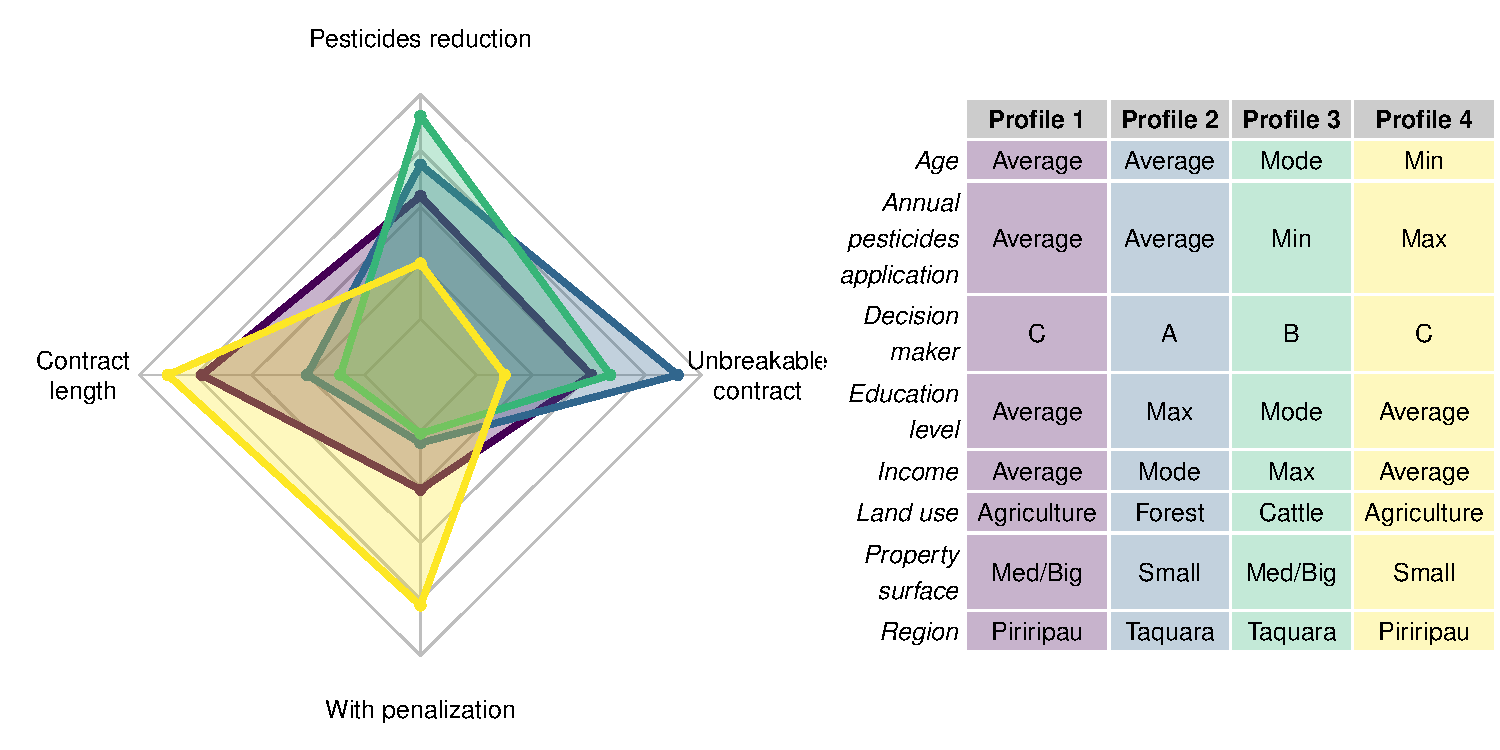
\includegraphics[width=\textwidth]{figures/spider.pdf}\\
 \caption{Spider chart for four variables based on the four most
          frequent profiles and their model coefficients}
 \label{fig:spider}
\end{figure}

With \autoref{fig:spider} and \autoref{fig:spiders}, we see a clear
difference between the profiles, showing the impact of changing even
just a few features in a profile, in terms of model coefficients. Each
profile is highlighted in one direction/variable. In
\autoref{fig:spider} we see all of them together, and in
\autoref{fig:spiders}, side=by-side. In three of the four variables,
profile 4 presents the most extreme coefficients.

\begin{figure}[H]
 \centering
 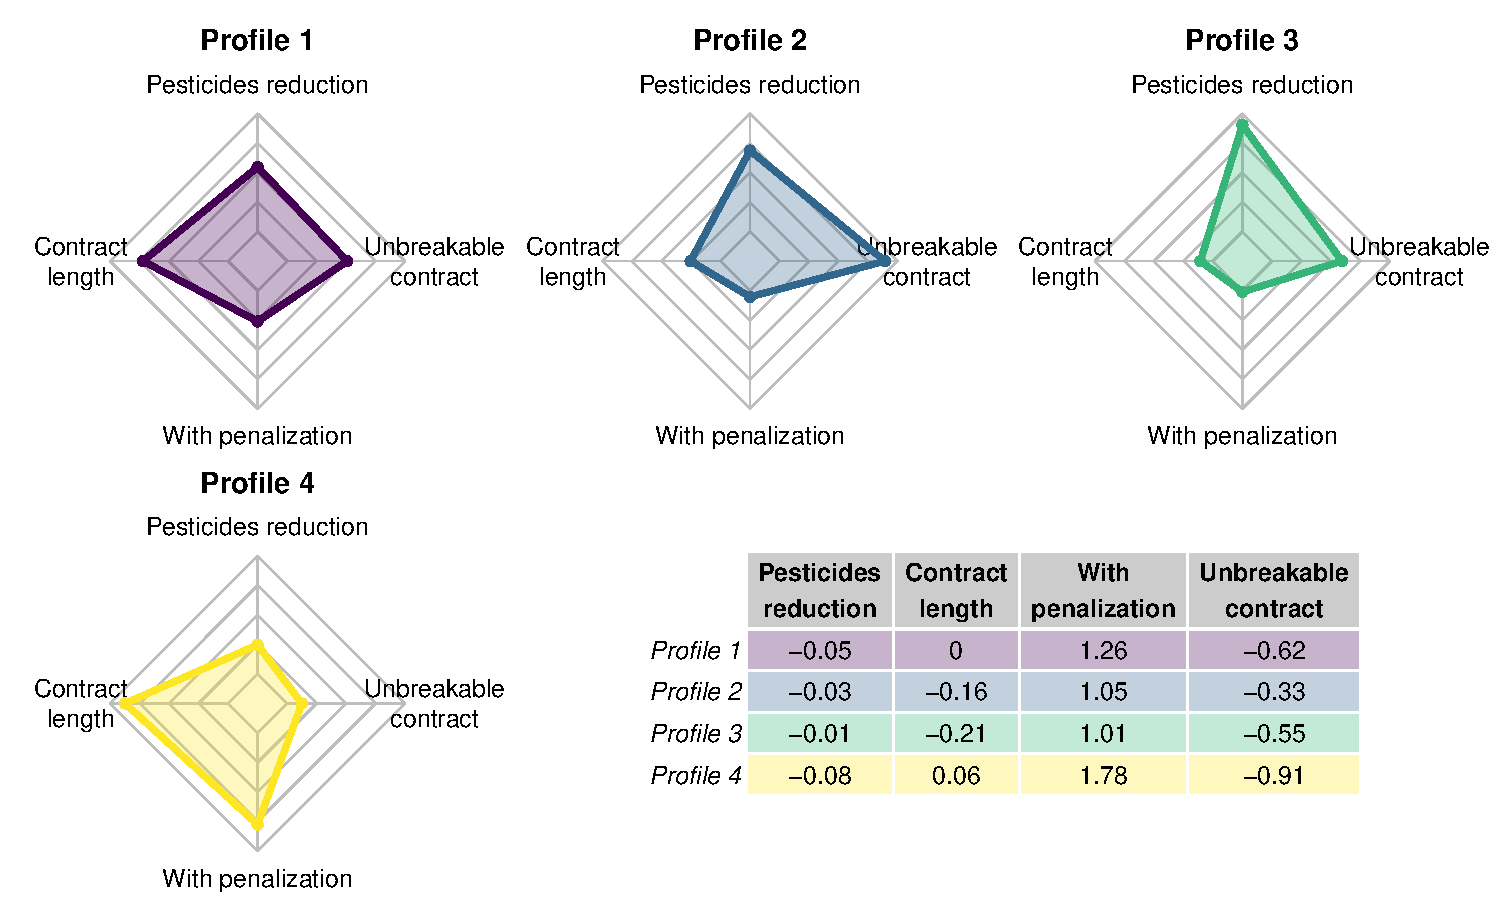
\includegraphics[width=\textwidth]{figures/spiders.pdf}\\
 \caption{Spider charts for four variables based on the four most
          frequent profiles and their model coefficients}
 \label{fig:spiders}
\end{figure}

\section*{WTA profit}
\addcontentsline{toc}{section}{WTA profit}

\begin{figure}[H]
 \centering
 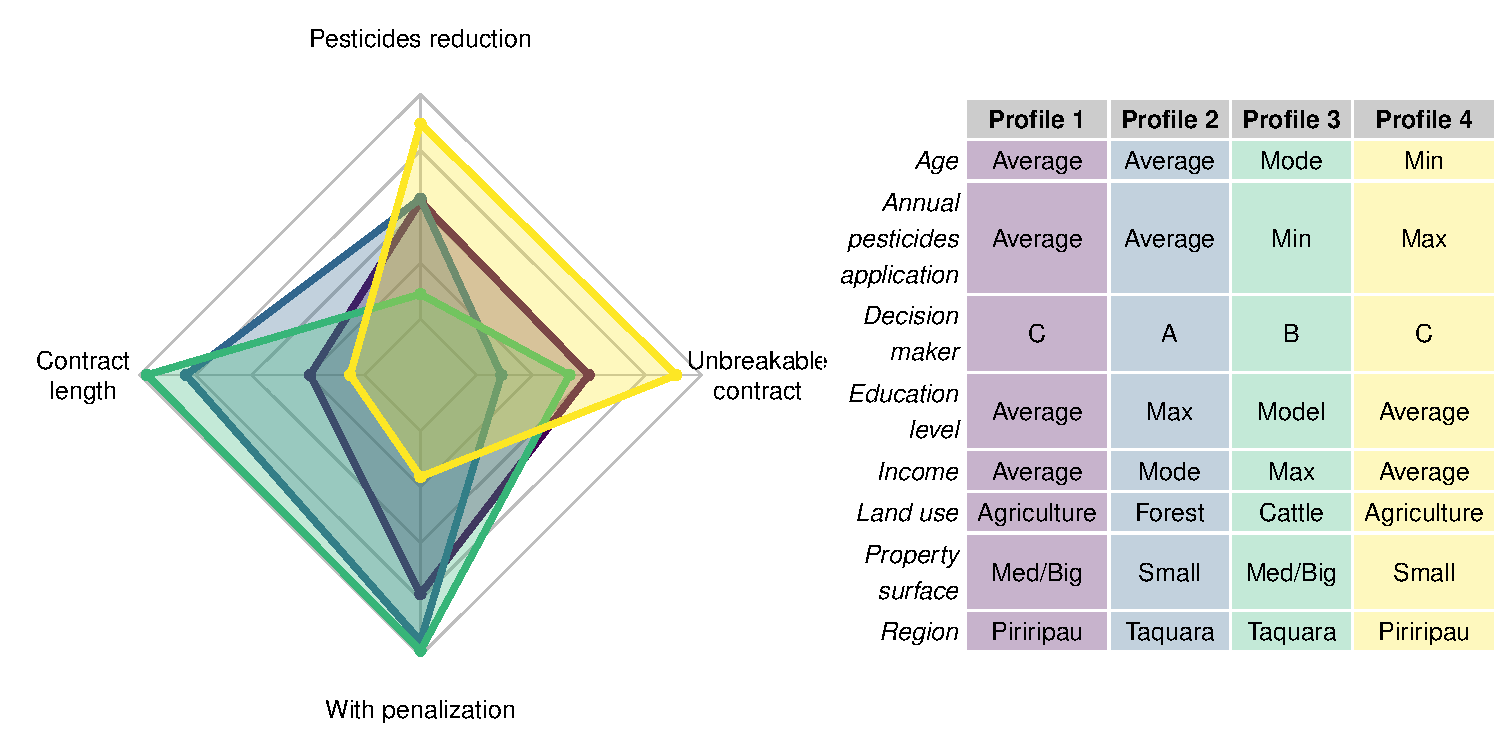
\includegraphics[width=\textwidth]{figures/spider_wta.pdf}\\
 \caption{Spider chart for four variables based on the four most
          frequent profiles and their WTA profits}
 \label{fig:spider_wta}
\end{figure}

In \autoref{fig:spider_wta} and \autoref{fig:spiders_wta}, we now look
at the WTA profits per variable and profile. We can still see clear
differences between the profiles, with each one highlighting a different
variable. Again, the most extremes values are obtained with profile 4.

\begin{figure}[H]
 \centering
 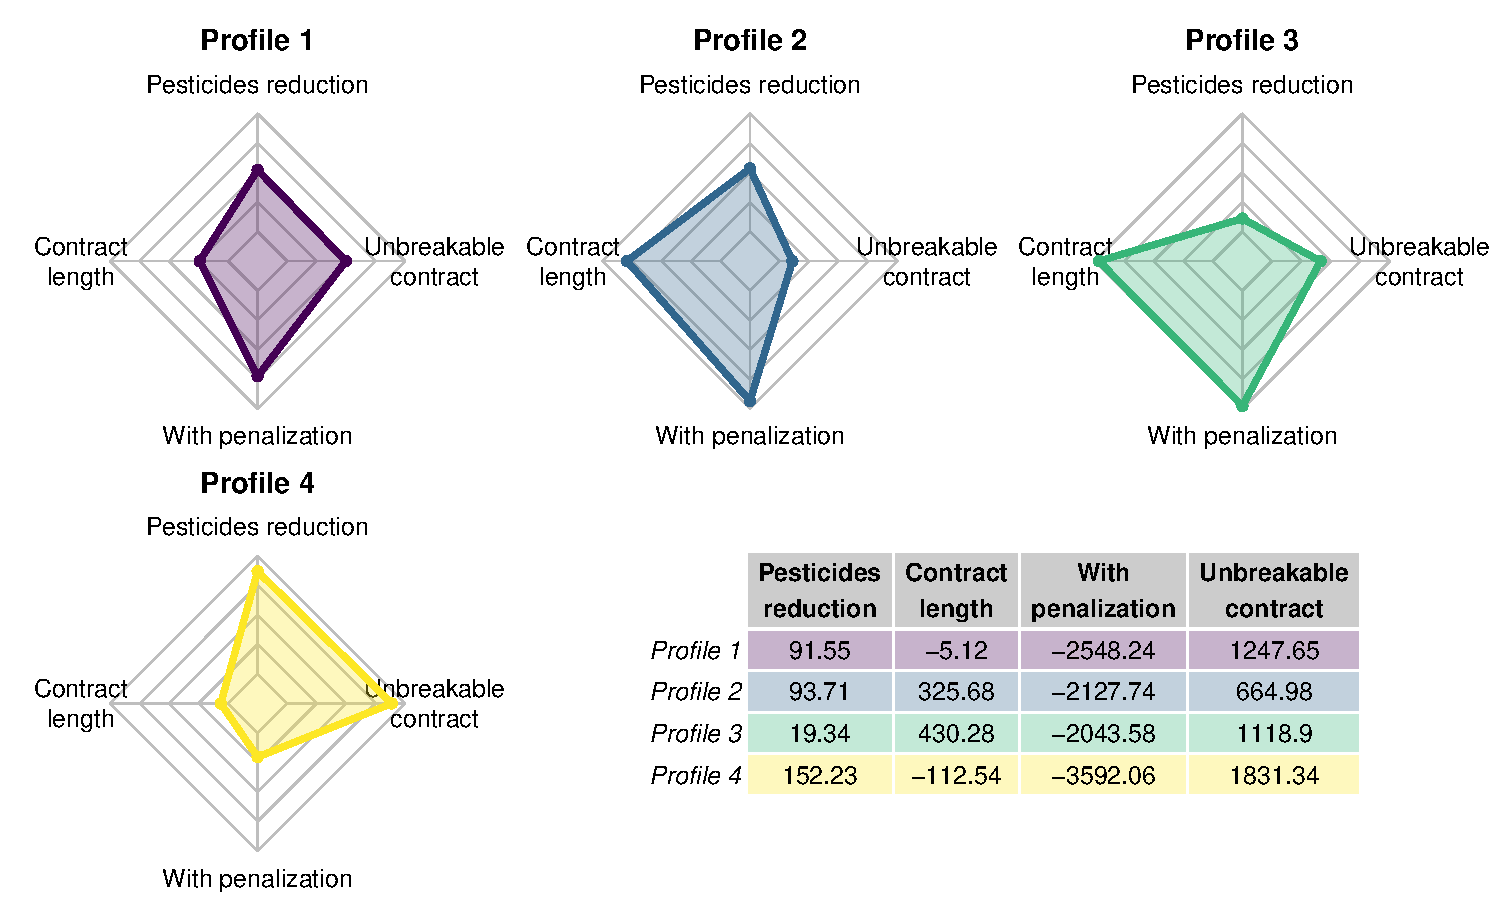
\includegraphics[width=\textwidth]{figures/spiders_wta.pdf}\\
 \caption{Spider charts for four variables based on the four most
          frequent profiles and their WTA profits}
 \label{fig:spiders_wta}
\end{figure}

\section*{Scenarios}
\addcontentsline{toc}{section}{Scenarios}

In \autoref{fig:scenarios}, we have the cost for each of the four
profiles in six different scenarios. We see that depending on the
scenario, the profiles behaviors vary considerably, being very difficult
to state any pattern.

\begin{figure}[H]
 \centering
 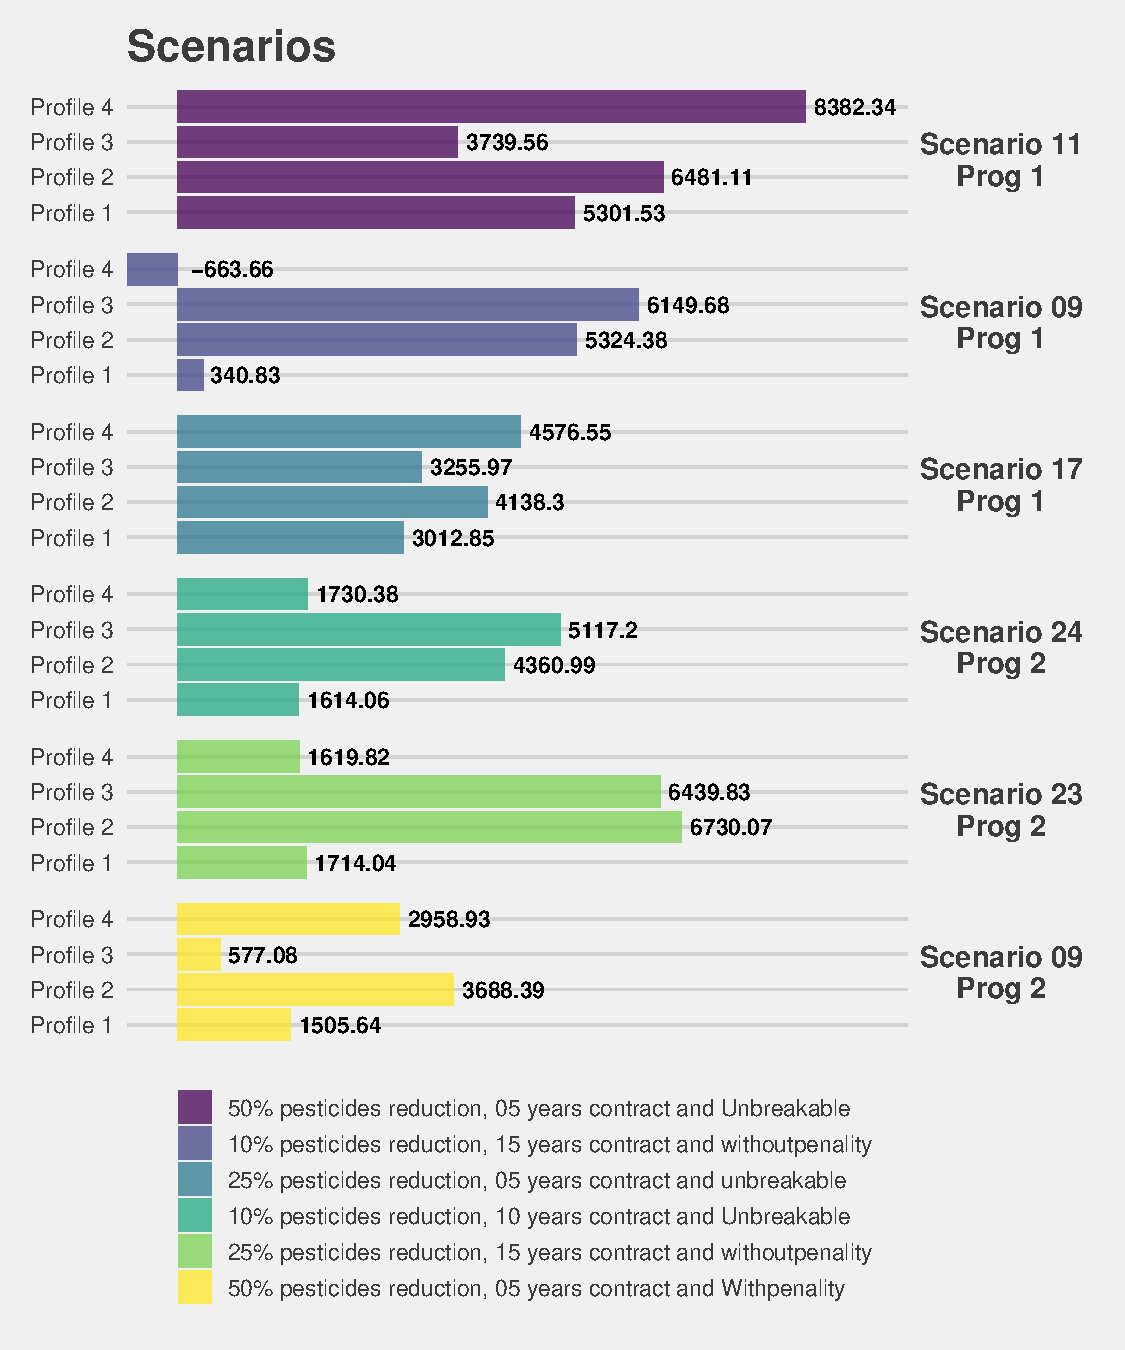
\includegraphics[width=0.85\textwidth]{figures/scenarios.pdf}\\
 \caption{Scenarios per the four most frequent profiles}
 \label{fig:scenarios}
\end{figure}

\section*{Model formula}
\addcontentsline{toc}{section}{Model formula}

\end{document}
